\documentclass[a4paper,11pt]{article}

\usepackage[hidelinks]{hyperref}
\usepackage[font={small}]{caption}
\usepackage{graphicx}
\usepackage{poltakmacros}           % Personal macros included in file 'poltakmacros.sty'.
\usepackage{geometry}

\geometry{margin=2cm}


\author{Jonathan Poltak Samosir}
\title{FIT3143 Assignment 2}


\begin{document}

\maketitle
\thispagestyle{empty}

\begin{abstract}
\end{abstract}
\smallskip
\noindent \textbf{Keywords.} blah, blah, blah
\newpage
\pagenumbering{roman}
\tableofcontents
\newpage

\pagenumbering{arabic}

% TODO: Split sections into different files
\section{Introduction} % (fold)
\label{sec:introduction}

% section introduction (end)


\section{Introduction to the multi-core CPU} % (fold)
\label{sec:introduction_to_the_multi_core_cpu}

\subsection{The central processing unit} % (fold)
\label{sub:the_central_processing_unit}
The central processing unit --- hereby referred to as the CPU --- is a fundamental piece of hardware within modern computers that handles
the fetching, decoding and execution of each instruction of a computer program~\cite{web:CPUWiki}. It handles the processing
of these instructions through the use of two key components: the arithmetic logic unit --- hereby referred to as the ALU
--- for basic arithmetical and logical operations, and the control unit --- hereby referred to as the CU --- for the input/output
operations between the CPU and memory, along with the overall control of the fetch, decode and execute cycle. Given the
physical hardware constraints, only a single instruction may be processed at any given time by a CPU.
% subsection the_central_processing_unit (end)

\subsection{The multi-core CPU} % (fold)
\label{sub:the_multi_core_cpu}
To define the multi-core CPU, it is perhaps important to first define the term ``core''. Like many terms in the area of computing,
the term ``core'' is often misused or used with many different meanings attached to it. For the purposes of this paper, the
term ``core'' simply refers to actual CPUs as defined in~\sectref{sub:the_central_processing_unit}.

Given this definition of a core, the multi-core CPU can simply be defined as a piece of computing hardware that contains
two or more cores. As the multi-core CPU contains more than one core, rather than being constrained to processing a single
instruction at any given time, in theory it is possible to be processing $n$ instructions on an $n$-core CPU at any given time.

Given what multi-core CPU hardware makes possible, since their introduction to consumers in the early 2000s, the multi-core
CPU has changed the way programmers design their programs to take advantage of hardware. Programs that are designed with
code concurrency in-mind now have advantages that were only ever available previously on systems that have multiple physical
CPU chips.
% subsection the_multi_core_cpu (end)

\subsection{Multi-core CPU architecture} % (fold)
\label{sub:multi_core_cpu_architecture}
The newest evolutions in multi-core CPU architecture families in modern consumer computing are arguably Intel's
``Haswell'' and AMD's ``Steamroller'' lines of processors.

Intel's Haswell is the fourth generation of their ``Core'' line of multi-processors, that places a larger focus on reducing power-consumption and improving performance of their on-chip graphics processing unit, or GPU~\cite{web:ForbesHaswell}. This point, specifically, will be elaborated on in further detail in later sections.

AMD's Steamroller architecture is the third evolution of AMD's ``Bulldozer''
architecture, a direct competitor to Intel's Haswell architecture implemented
in their ``Core'' line of multi-core processors. Steamroller placed a larger focus on improving parallelism between the available cores~\cite{web:AMDCCCSlides}, while also attempting to address competitor Intel's area of dominance--- power
consumption.
% subsection multi_core_cpu_architecture (end)

\subsection{Intel Haswell Core i7-4770K architecture} % (fold)
\label{sub:intel_haswell_architecture}
As an example of a Haswell CPU to specifically look at, we will take Intel's
current flagship enthusiast model Haswell quad-core processor, the Core i7-4770K. While having four cores all on the same chip, this Core i7 also
contains its own GPU on the chip. The Haswell i7 is a multi-level cache CPU, with each core having three levels of cache memory
available to it; from fastest to slowest: L1, L2 and L3. Each core has its own
dedicated 64 KB of L1 cache (split into 32 KB halves for separate data and instruction caches), 256 KB of L2 cache and all the cores share a much slower 8 MB of L3 cache~\cite{web:TomsHWCorei7}. The overall layout of the chip, as explained here, can be seen in~\figref{fig:haswell-layout}.

\begin{figure}[h]
  \centering
  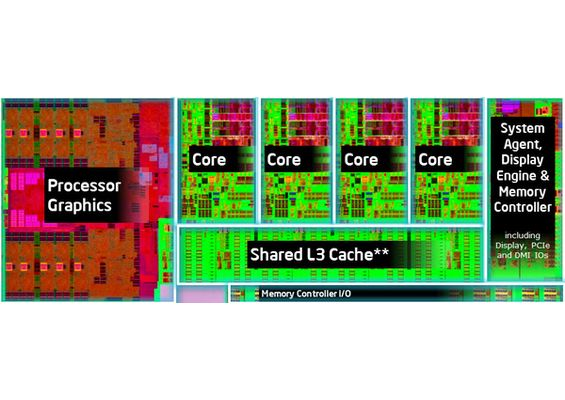
\includegraphics[scale=0.5]{img/haswell-layout}
  \caption{The Intel Core i7-4770K quad-core CPU die layout.~\cite{web:TomHWCorei7DiePic}}
\label{fig:haswell-layout}
\end{figure}

Something of note is how the i7-4770K enables pipelining of operations with its hardware. Before proceeding into pipeling, it is important to touch on the differences between instructions and operations: Instructions are decoded by the CPU into atomic parts which are known as micro-operations which use and require specific resources. These micro-operations are then queued into the ``Unified Reservation Station'' (URS) where they wait until their resources are available. The micro-operations are then dispatched from the URS to the appropriate execution port. This is all done ``out of order'' where operations are just dispatched whenever possible, rather than in a pre-determined order when there is no resource dependencies between operations~\cite{book:Corei7PerfAnalysis}. Hence, this is the specific implementation of CPU pipelining that is enabled on the Haswell architecture. As can be seen from~\figref{fig:haswell-new-ports}, Haswell has eight distinct execution ports, each supporting different operations. This allows a maximum of eight independent micro-operations to be executed each clock cycle~\cite{web:TomsHWCorei7}.

\begin{figure}[h]
  \centering
  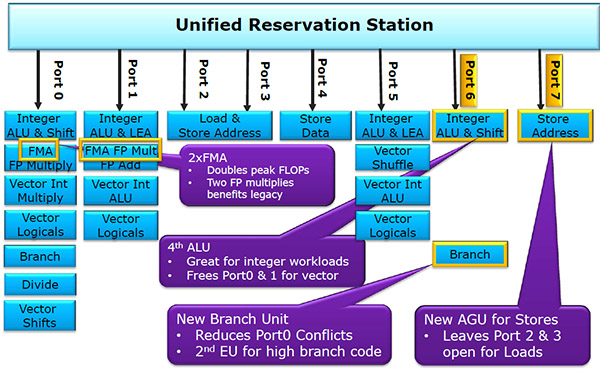
\includegraphics[scale=0.5]{img/new-ports}
  \caption{Shows how operation out of order execution pipelining works in the Intel Core i7-4770K~\cite{web:TomsHWCorei7}. The Unified Reservation Station can be seen along with the i7's eight execution ports. New hardware additions to the Haswell architecture highlighted.}
\label{fig:haswell-new-ports}
\end{figure}
% subsection intel_haswell_architecture (end)

\subsection{AMD Steamroller/Kaveri architecture} % (fold)
\label{sub:amd_steamroller_architecture}
As an example of a Steamroller-based CPU, we will look at AMD's current flagship A10-7850K processor, which is based on the third evolution of the Steamroller architecture, codenamed ``Kaveri''.

Something of note when looking at modern AMD processors is to note AMD's use of the marketing term ``APU'' --- short for Accelerated Processing Unit. This is essentially AMD's term for a GPU and CPU dual-offering on the same die~\cite{web:AMDAPU}, similar to what is provided by Intel's Haswell line of processors (as elaborated on in~\sectref{sub:intel_haswell_architecture}).

The die layout for the Kaveri processors is quite different to what we have previously seen with Intel's Haswell processors. The most obvious difference is that the majority of the die is taken up by the GPU

\begin{figure}[h]
  \centering
  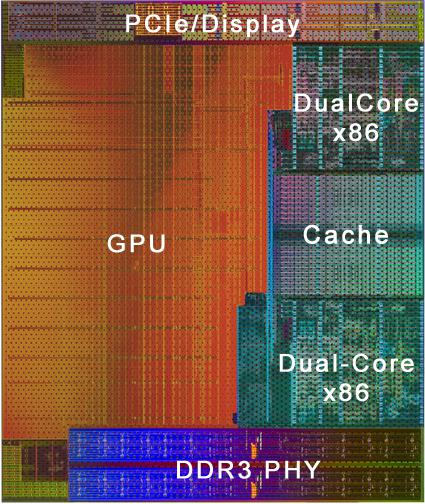
\includegraphics[scale=0.5]{img/kaveri_die}
  \caption{The AMD Kaveri quad-core CPU die layout.~\cite{web:Guru3dKaveri}}
\label{fig:kaveri-layout}
\end{figure}
% subsection amd_steamroller_architecture (end)




% section introduction_to_the_multi_core_cpu (end)


\section{Programming the multi-core CPU} % (fold)
\label{sec:programming_the_multi_core_cpu}

% section programming_the_multi_core_cpu (end)


\section{Introduction to the GPU} % (fold)
\label{sec:introduction_to_the_gpu}

% section introduction_to_the_gpu (end)


\section{Differences in programming the GPU} % (fold)
\label{sec:differences_in_programming_the_gpu}

% section differences_in_programming_the_gpu (end)


\section{Parallelism in the multi-core CPU and GPU} % (fold)
\label{sec:parallelism_in_the_multi_core_cpu_and_gpu}

% section parallelism_in_the_multi_core_cpu_and_gpu (end)


\section{Conclusion} % (fold)
\label{sec:conclusion}

% section conclusion (end)


\bibliographystyle{acm}
\bibliography{report}

\end{document}
